%%%%%%%%%%%%%%%%%%%%%%%%%%%%%%%%%%%%%%%%%%%%%%%%%%%%%%%%%%%%%%%%%%%%%%%%%%%%%%%
%
% 876729-ELEN40XX-2025.tex
%
%                       Kgadile E. Masemola (29 March 2025)
%
%                       Sample Paper for ELEN40XXA 2025
%
%						edited by numbat24.04, 2025-03-30
%
%%%%%%%%%%%%%%%%%%%%%%%%%%%%%%%%%%%%%%%%%%%%%%%%%%%%%%%%%%%%%%%%%%%%%%%%%%%%%%%%

\documentclass[a4paper,12pt]{article}
\usepackage[a4paper,left=3cm,right=3cm,top=2.5cm,bottom=2.5cm]{geometry}
%\usepackage{fullpage}
\usepackage{graphicx}
%\usepackage{gensymb}
\usepackage{eqnarray,amsmath, amssymb}
\usepackage{bookmark}
\usepackage{hyperref}
\usepackage{listings}
\usepackage{enumitem}
\usepackage{booktabs}
\usepackage{longtable}
\usepackage{arydshln}
%\usepackage{changepage}
%\usepackage{empheq}
%\usepackage[most]{tcolorbox}
%\usepackage[table]{xcolor}
\usepackage{geometry}
\geometry{margin=1in}
\usepackage{booktabs}

\usepackage{caption}
\usepackage{subcaption}
\usepackage{enumitem}

%\makeatletter
%\renewcommand\@seccntformat[1]{}
%\makeatother

%
% All KEM's macros and goodies (some shameless borrowing from SPL)

%
% PDF Info
%
\hypersetup{pdfinfo={
Title = {ELEN4006-MeasurementS' Lab-Report},
Author = {Kgadile "Naar-Kie" Masemola},
CreationDate = {D:202504030836},
%ModDate = {D:202409040530},
Subject = {ELEN40XXA Paper Format, 2025},
Keywords = {numbat24.04}
}}

%%%%%%%%%%%%%%%%%%%%%%%%%%%%%%%%%%%%%%%%%%%%%%%%%%%%%%%%%%%%%%%%%%%%%%%%%%%%%%%%%%%%%%%%%%%%


%%%%%%%%%%%%%%%%%%%%%%%%%%%%%%%%%%%%%%%%%%%%%%%%%%%%%%%%%%%%%%%%%%%%%%%%%%%%%%%


\begin{document}
\begin{titlepage}
\begin{figure}
\centering

\includegraphics[scale=0.5]{witseie100logo.png}  
\end{figure}
\title{Hand Movement Distance Measurement System\\
\large \underline{Laboratory Assignment}}
\author{Kgadile E. Masemola (\underline{876729})\\ ELEN4006A - Measurement Systems}
\date{April 22, 2025}
\maketitle
%%%%%%%%%%%%%%%%%%%%%%%%%%%%%%%%%%%%%%%%%%%%%%%%%%%%%%%%%%%%%%%%%%%%%%%%%%%%%%%
%
\begin{abstract}
This report presents the design, implementation, and evaluation of a hall effect-based displacement measurement system. Using a neodymium magnet and hall effect sensor, the system accurately measures small hand movements for small distances, not suitable for wrist flexion rehabilitation monitoring. The results highlight the sensor's high linearity, accuracy, and minimal loading effects. The high-level solution involves a wrist-worn sensor and finger-worn magnet feeding an microcontroller measurement system that outputs a quantitative measure of finger displacement, thereby addressing the need for objective tracking of rehabilitation progress.
\end{abstract}
\end{titlepage}

%\maketitle
%\thispagestyle{empty}\pagestyle{empty}
%\keywords{myoelectric, EMG}


%%%%%%%%%%%%%%%%%%%%%%%%%%%%%%%%%%%%%%%%%%%%%%%%%%%%%%%%%%%%%%%%%%%%%%%%%%%%%%%
%
\section{Introduction}
Stroke rehabilitation is significantly enhanced by quantitative monitoring of patient hand movements, as it guides rehabilitation strategies and accelerates recovery \cite{langhorne2011stroke}. The tracking of hand movements during stroke rehabilitation aids clinicians in adjusting therapy methods, thereby accelerating patient recovery \cite{veerbeek2014effects}. This paper aims to design a wrist wrist flexion movement measurement system. The system utilises a hall effect sensor and neodymium magnet, taking advantage of changes in magnetic flux density to produce an analog voltage proportional to displacement \cite{popovic2013hall}.\\
Section 2 to 3 shows the design process of the system. Performance and analysis are discussed in section 4 and 5. This is followed by group reflection and summary.

%%%%%%%%%%%%%%%%%%%%%%%%%%%%%%%%%%%%%%%%%%%%%%%%%%%%%%%%%%%%%%%%%%%%%%%%%%%%%%%
%
\section{Design Specification and High-level Solution}
Design specifications are shown in Table 1. 
\begin{table}[ht]
\centering
\caption{Design specifications.}
\begin{tabular}{|>{\centering\arraybackslash}p{2.2cm}|>{\centering\arraybackslash}p{2.5cm}|>{\centering\arraybackslash}p{2cm}|>{\centering\arraybackslash}p{1.5cm}|>{\centering\arraybackslash}p{2.5cm}|>{\centering\arraybackslash}p{2.5cm}|}
\hline
\textbf{Input Range} & \textbf{Bandwidth} & \textbf{Accuracy (FSD)} & \textbf{IP rating} & \textbf{Op. Temp.} & \textbf{Output range} \\
\hline
0 - 212 mm & $\leq 30 \text{Hz}$ & $>95\%$ & 22 \cite{coutts2025ingress}  & $-40$ - $120$ \textdegree{}C & $0$ - $5 \text{V}$  \\
\hline
\end{tabular}
\end{table}
Input range is for an average human hand which measures 18cm from wrist to middle finger \cite{guerra2014hand}. The arc length for a typical wrist of 70\textdegree{} is 212mm. Bandwidth is designed according to a human hand motion which is typically $<$ 2 Hz, we want to measure up to the 15th harmonic for extreme unusual movements \cite{rohrer2002movement}. Accuracy of $5\%$ of full scale output change sufficient to detect small improvements in range. calculated from datasheet of sensor datasheet and operational temperature which covers the ambient value at typical rehabilitation clinics \cite{primex2023}. The output voltage range(0 - 5V) from sensor aligns with Arduino input range. Arduino Uno is selected based on availability and it's ability to do these kinds of projects as used here \cite{wiyono2021simulation}\\
Figure \ref{fig:measure_diag} shows a diagram of how the measurement system will work based on wrist movement as per specification. This type of wrist movement is used as rehabilitation exercise in clinics \cite{yuzer2017randomized}.
\begin{figure}[!ht]
    \centering
    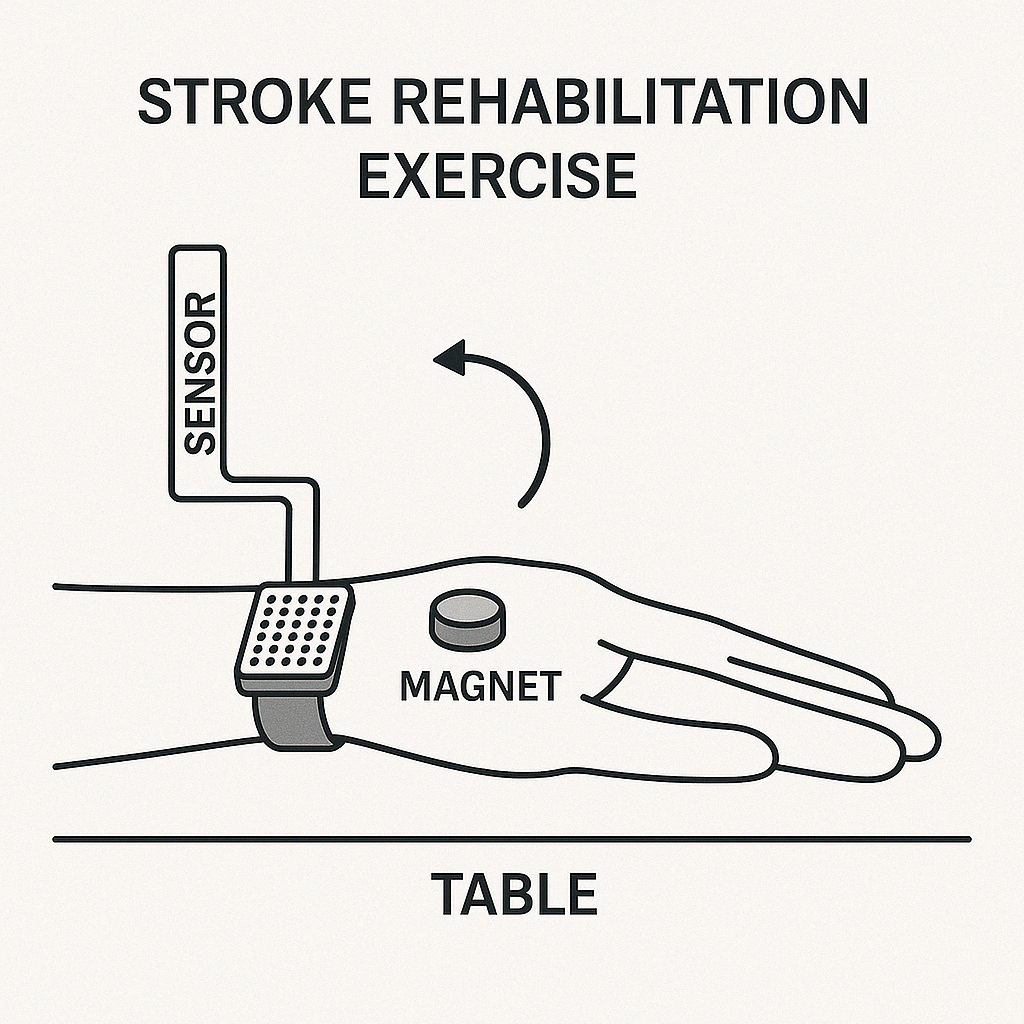
\includegraphics[width=0.3\textwidth]{diagram-Measure.png}
    \caption{Diagram of the hand distance measurement system}
    \label{fig:measure_diag}
\end{figure}
A high-level block diagram based on the Bentley model is shown in Figure \ref{fig:bentley}. As the wrist moves, the sensor output shifts from 2.5 to 5V. An analog signal conditioning stage removes the 2.5 V bias and amplifies the signal (typically 2.5 - 5V) to maximise the ADC resolution . The microcontroller processes this data and outputs the distance in mm for display on a LCD screen.

\begin{figure}[!ht]
    \centering
    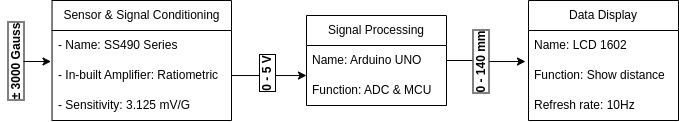
\includegraphics[width=0.85\textwidth]{LabBentley.png}
    \caption{High level block diagram of the measurement system}
    \label{fig:bentley}
\end{figure}


%%%%%%%%%%%%%%%%%%%%%%%%%%%%%%%%%%%%%%%%%%%%%%%%%%%%%%%%%%%%%%%%%%%%%%%%%%%%%%%
%
\section{Detailed Design}
 The complete circuit diagram in Figure \ref{fig:cct_system} illustrates the full implementation, with design choices justified in the subsequent sections. 
\begin{figure}[!ht]
    \centering
    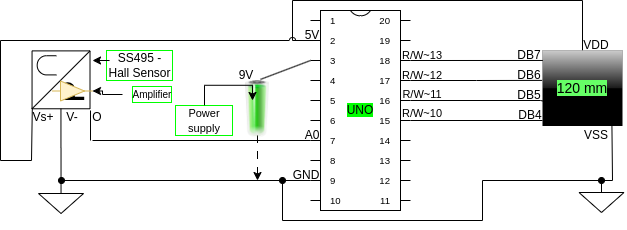
\includegraphics[width=0.8\textwidth]{LabCctDiagBlock.png}
    \caption{Complete circuit and high-level block diagram of the measurement system}
    \label{fig:cct_system}
\end{figure}


\subsection{Sensing element}
The sensing element comprises a Honeywell SS495A hall-effect sensor \cite{ti_datasheet} and neodymium magnet. These components are prescribed for this laboratory project. The sensor has a an in-built amplifying element that is at readable voltage values \cite{ti_datasheet}.

\subsection{Signal conditioning}
The sensor’s output can source or sink up to 1.5 mA  \cite{ti_datasheet}, and the input bias of the op amp is in the microamp range, so the sensor is not appreciably loaded by the amplifier. This was confirmed by observing no change in sensor output whether the op amp was connected or not. The op amp’s output drives the Arduino ADC input, which presents a small capacitance and a resistance of $\sim 100 \text{M} \Omega$ \cite{arduino}.

\subsection{Signal processing and Display}
We use a standard Arduino (e.g. Arduino Uno with ATmega328P) as the microcontroller for prototyping. It provides a 10-bit ADC and the convenience of the Arduino IDE for quick development. The Arduino’s analog input A0 reads the conditioned sensor voltage. With a 5 V reference, the ADC has a resolution of 5 V/1024 $\approx$ 4.88 mV per count \cite{hu2025adc}. This corresponds to roughly 0.5 mm of finger movement in our calibrated range, which is an acceptable resolution for this purpose \cite{kortier2014assessment}.\\ 
The microcontroller code continuously samples the analog input, applies a calibration conversion to translate the voltage to a distance, and then displays the result. The processed displacement data is displayed to an LED display in millimeters for the nurse and patient to view and record rehabilitation progress. The logical flow of the microcontroller processing is depicted in Figure \ref{fig:flow}.
\begin{figure}[ht]
    \centering
    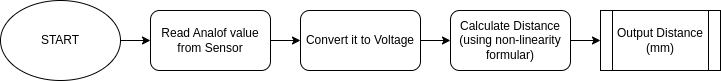
\includegraphics[width=0.8\textwidth]{LabMCUFlow.png}
    \caption{Flow diagram of microcontroller logic}
    \label{fig:flow}
\end{figure}
A simple calibration procedure is done initially: with the hand open, the output is set to 0 mm; with the finger fully bent to touch the sensor, the output distance is set to the known distance at contact. Intermediate distances can be calibrated by comparison against a ruler. 




%%%%%%%%%%%%%%%%%%%%%%%%%%%%%%%%%%%%%%%%%%%%%%%%%%%%%%%%%%%%%%%%%%%%%%%%%%%%%%%
%
\section{Performance Evaluation}
To evaluate the system, we conducted a series of bench-top tests with the assembled prototype. Hall sensor was placed on a breadboard, magnet moved by a slider to simulate finger motion. The testing results of the integrated system is shown in Figure \ref{fig:testres}. 
\begin{figure}[h]
\centering
\begin{subfigure}{0.5\textwidth}
  \centering
  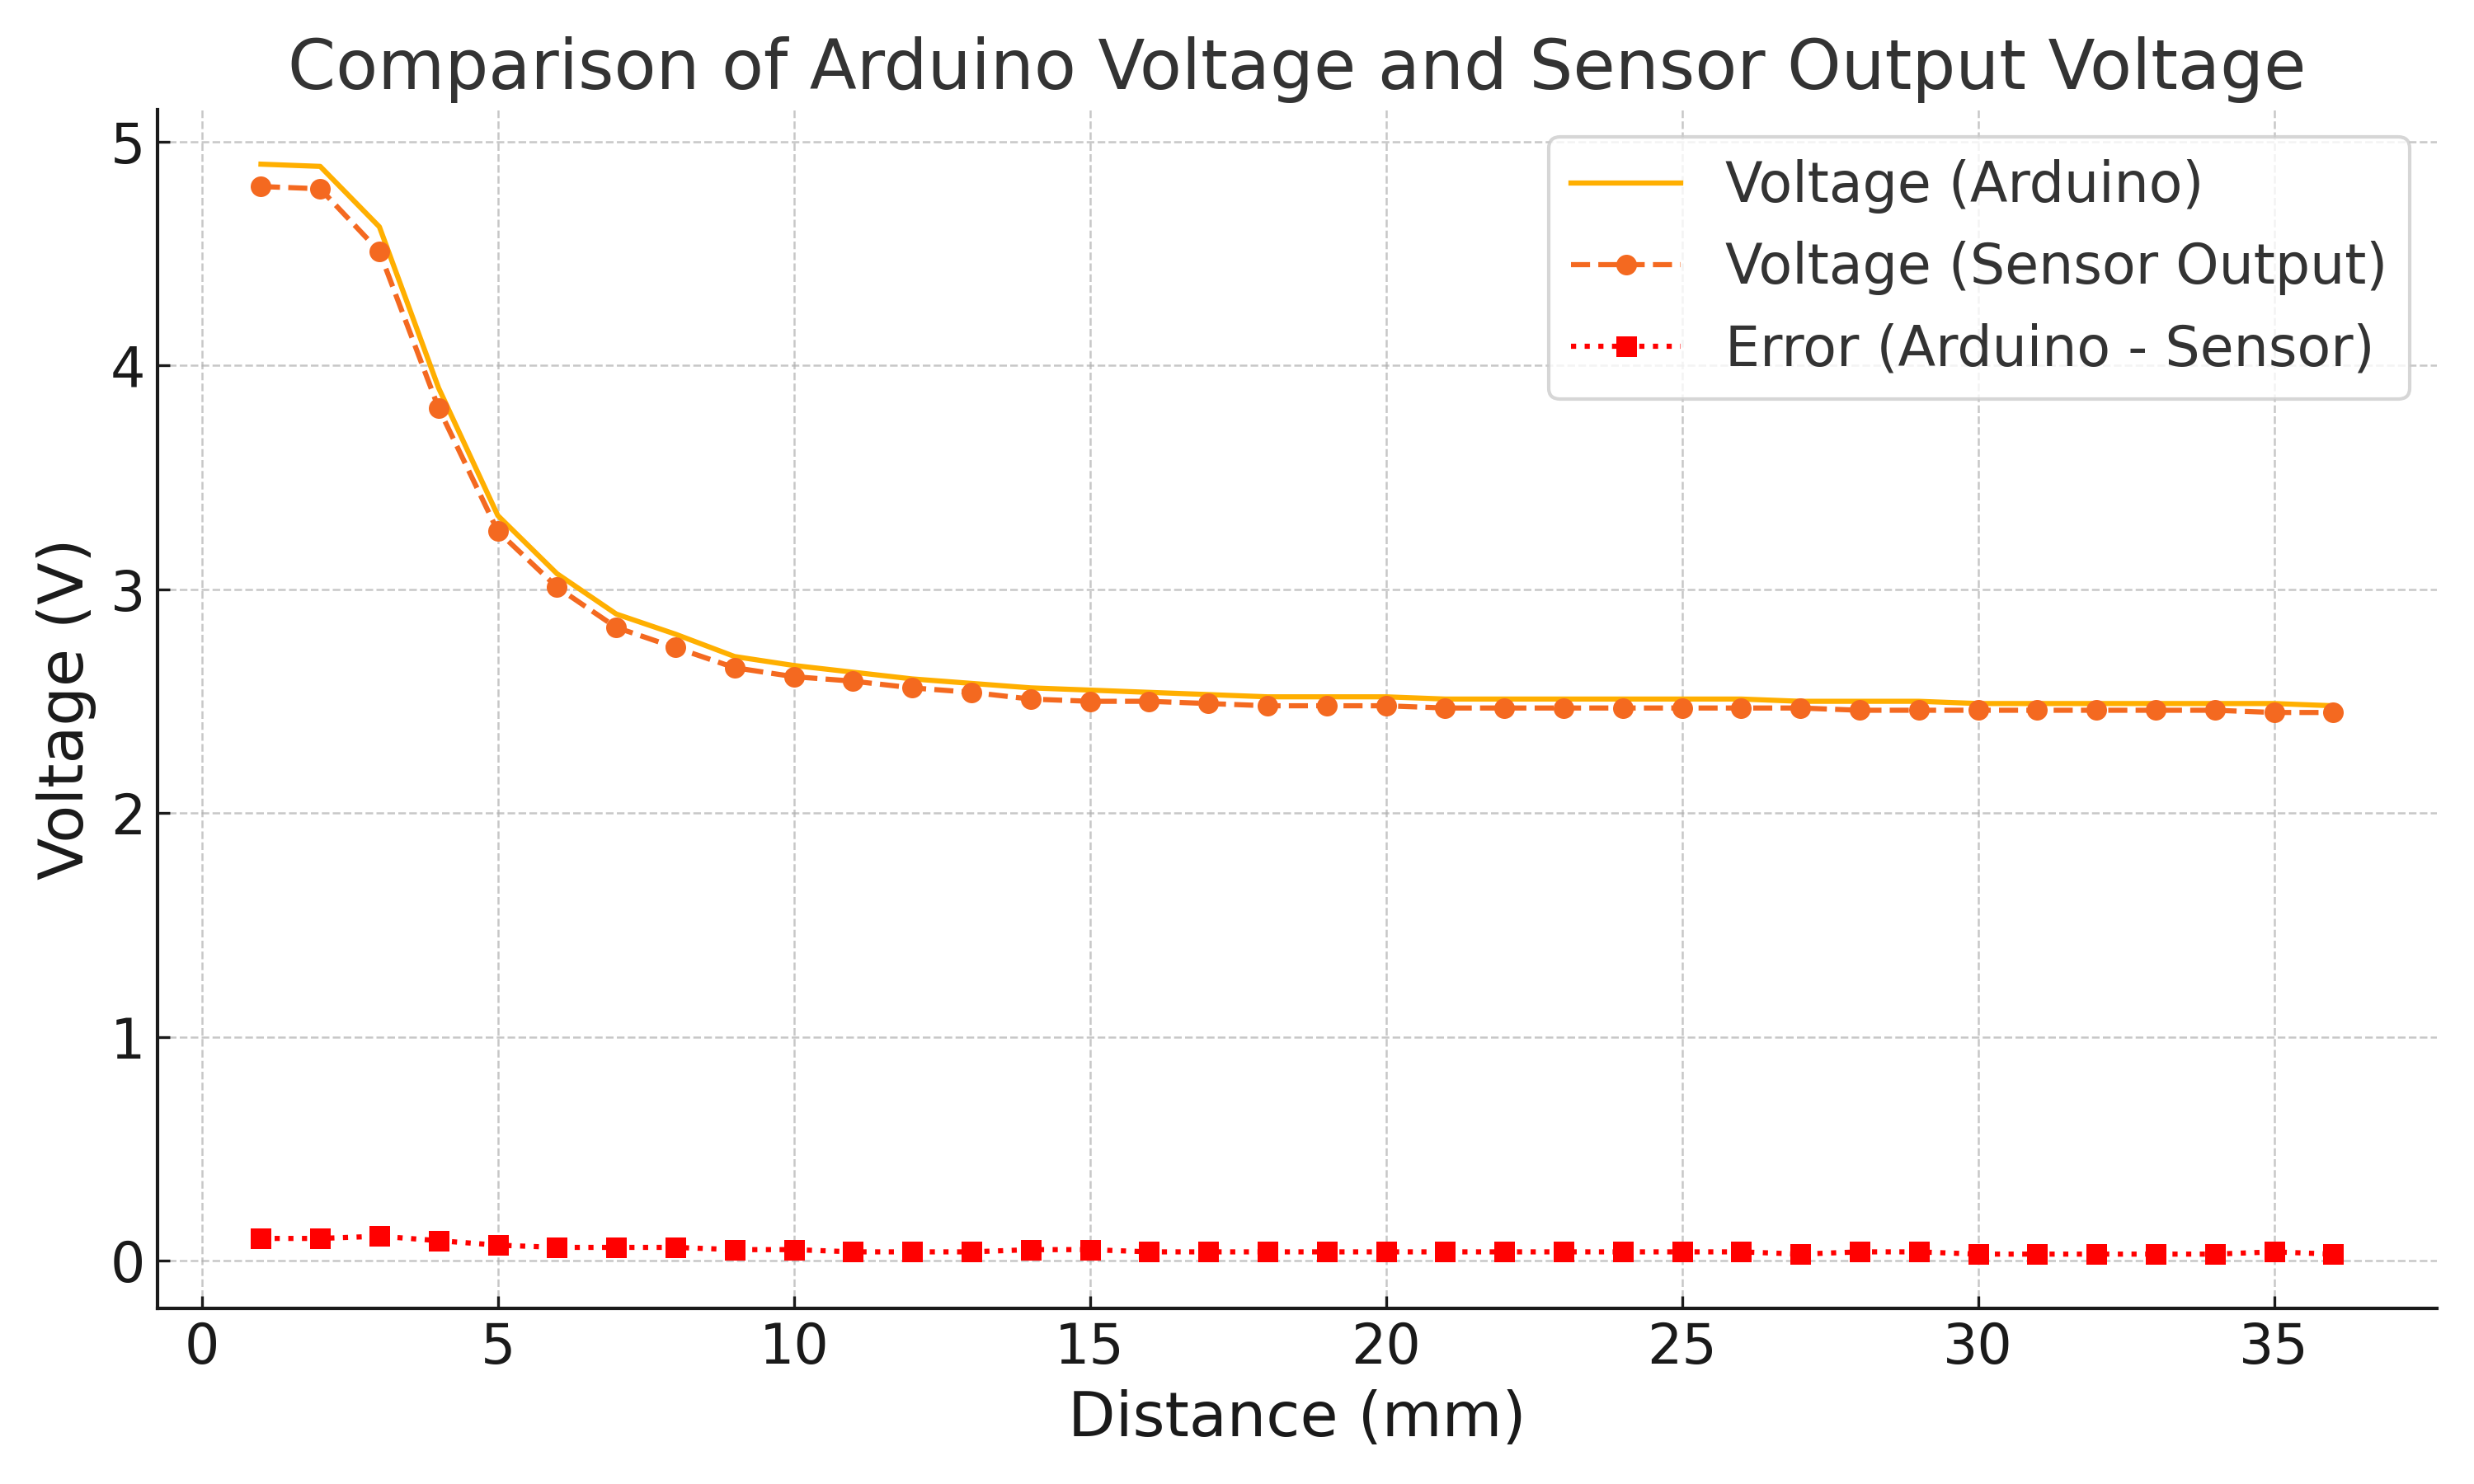
\includegraphics[width=\linewidth]{distvsvoltX2.png}
  \caption{Output Voltage vs Distance}
  \label{fig:voltdist}
\end{subfigure}\hfill
\begin{subfigure}{0.5\textwidth}
  \centering
  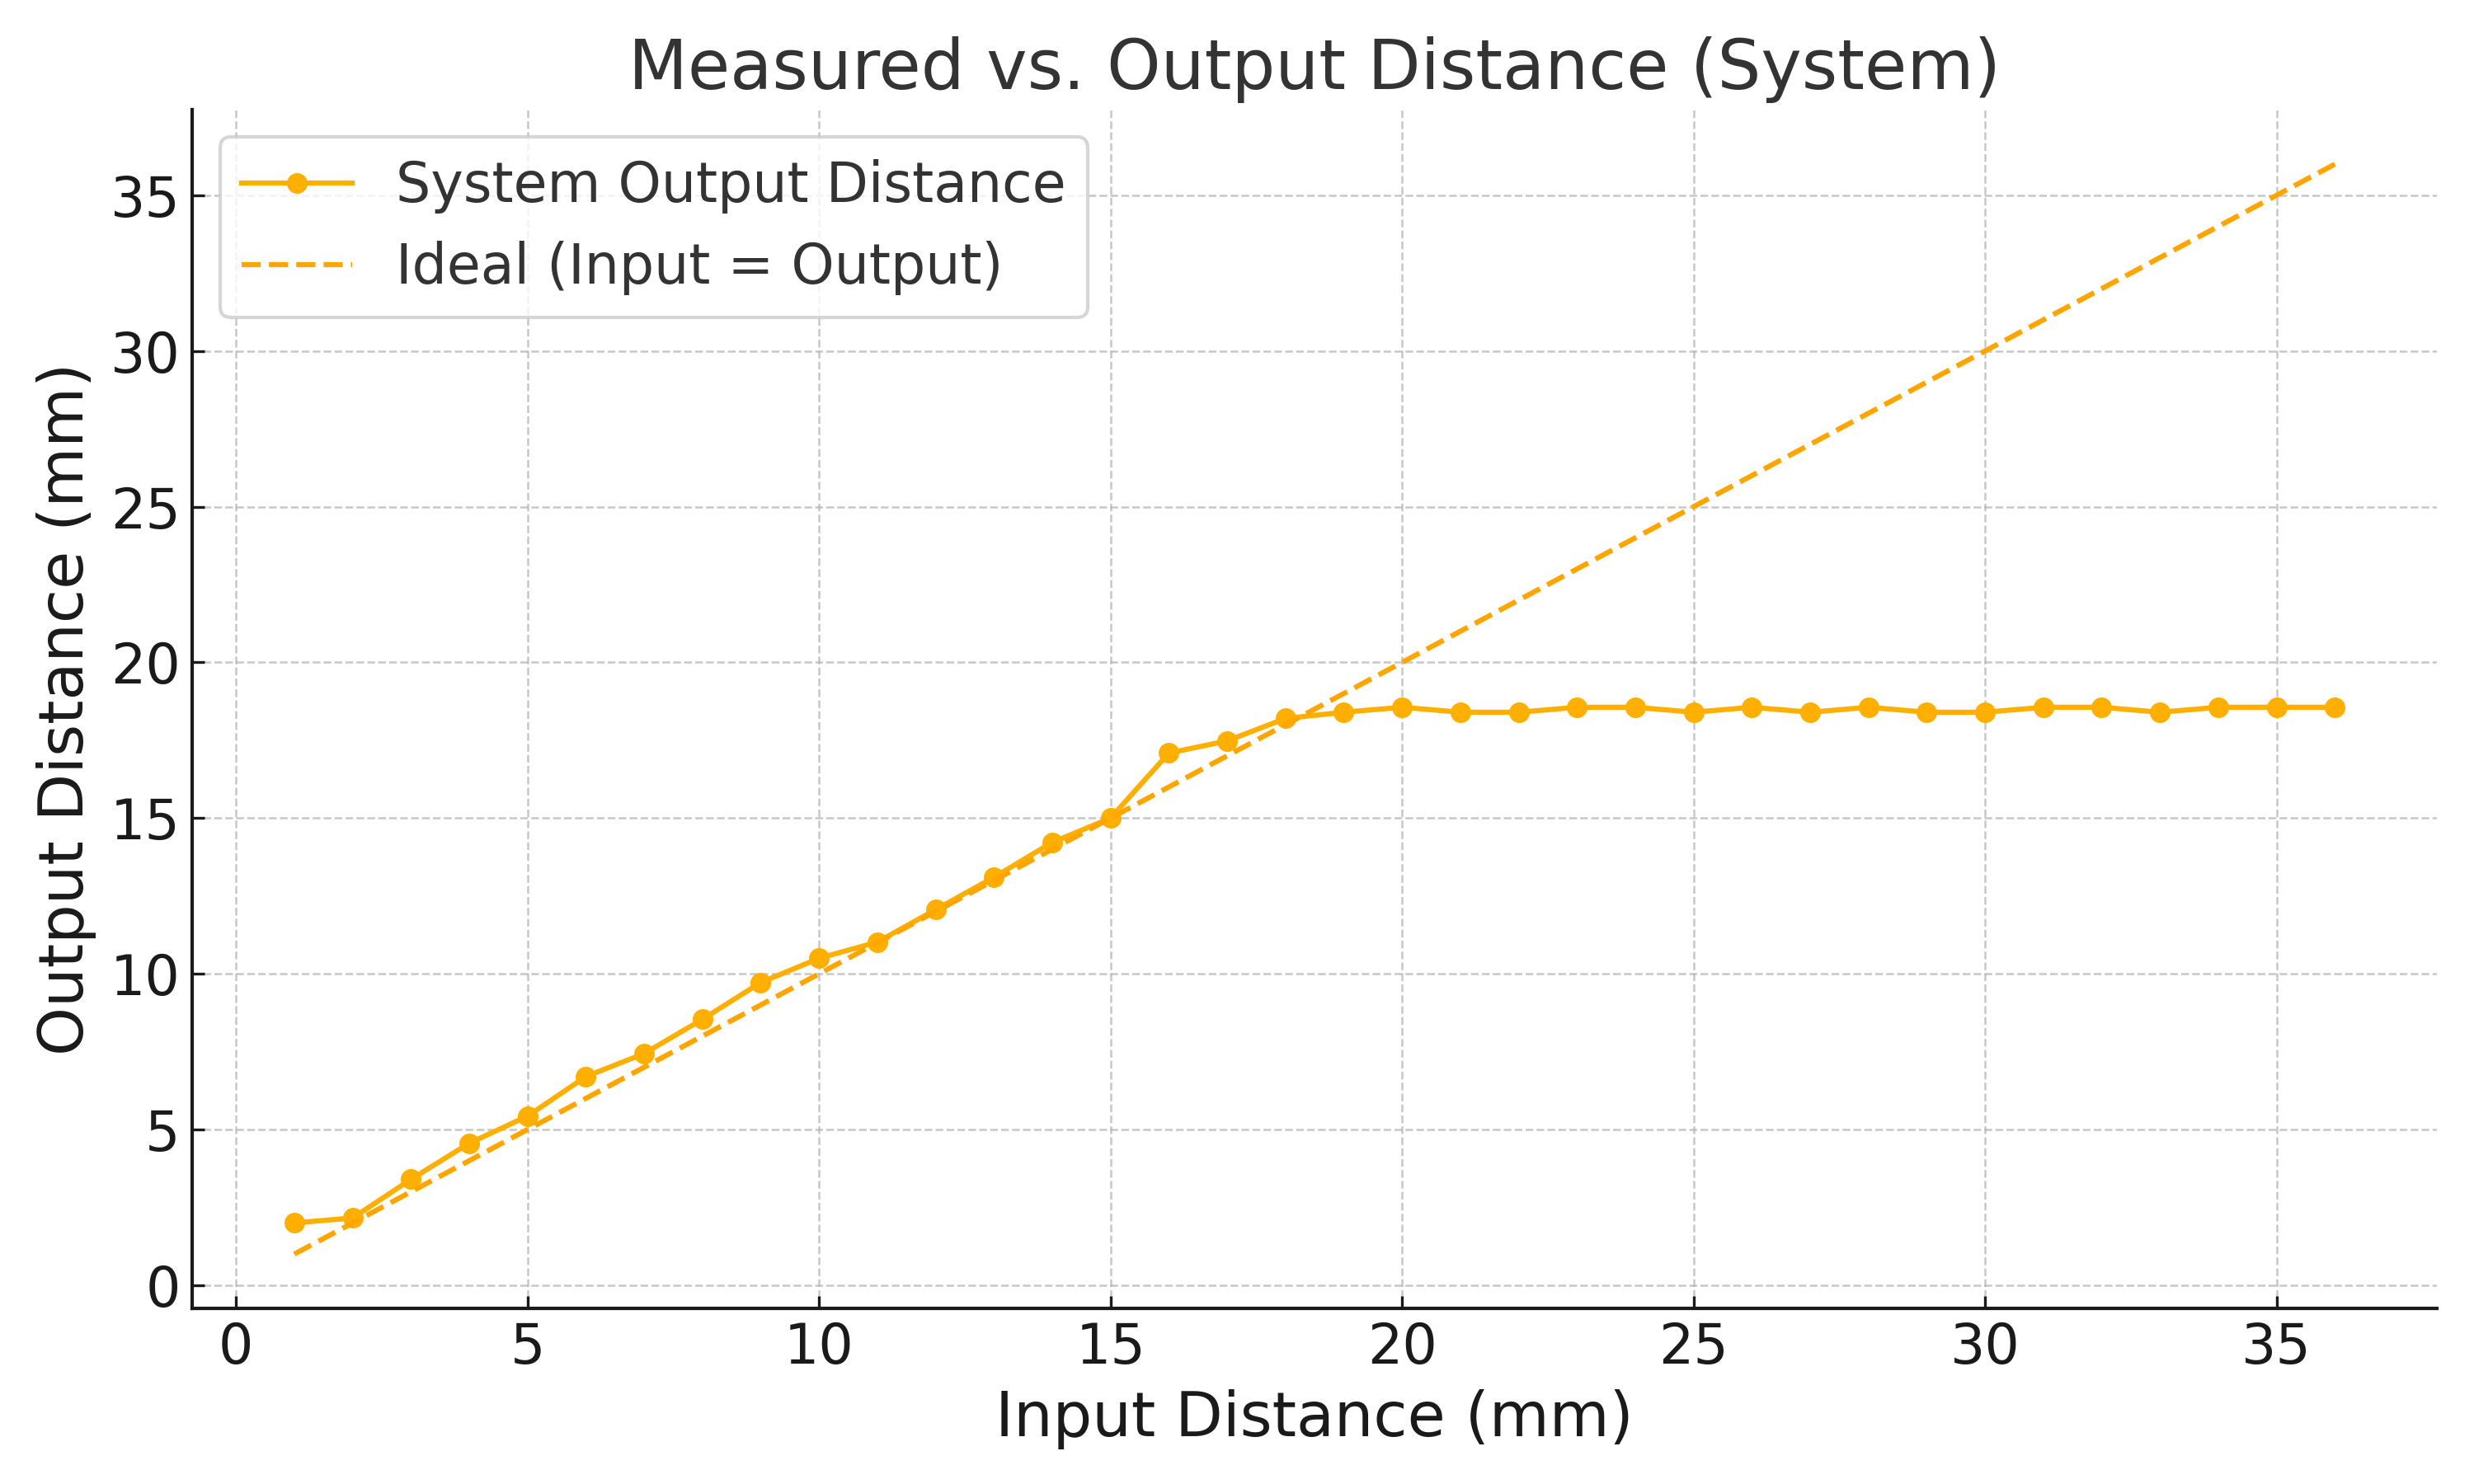
\includegraphics[width=\linewidth]{iodist.png}
  \caption{Input-Output distance comparison}
  \label{fig:distdit}
\end{subfigure}
\caption{Hand movement distance measurement system test results}
\label{fig:testres}
\end{figure}
Figure \ref{fig:voltdist} is showing the relationship between distance versus output voltage at the sensor and arduino ADC output. The corresponding error is relatively small, mostly $< 0.1$V, suggesting the Arduino's ADC is fairly accurate. This is due to ADC quantization error and possible reference voltage mismatch or board-level noise \cite{das_adc2020}. Graph in Figure \ref{fig:distdit} compares the system performance between real results and system results. The system tracks the input quite well up to $\sim 15$ mm, but then saturates near $18.4–18.56$ mm, indicating the sensor's sensitivity limit has been reached. The maximum error for the test input measurent is 17.44 mm at 36 mm. This is not acceptable for the movement tracking of wrist movement \cite{das_adc2020}.

\begin{itemize}
    \item \textbf{Sensor Sensitivity}: Estimated at 2.45 mV/Gauss (within 2\% of specification).
    \item \textbf{Bandwidth}: The SS495A sensor itself has a very fast response ($3 \mu$s rise time). the op amp (LM358) has a gain-bandwidth of $\sim 1$ MHz. The microcontroller sampling at $\sim 20$ Hz means the overall system bandwidth is limited by sampling to about 10 Hz (Nyquist), which is intentional. This is more than sufficient for capturing voluntary finger movements (which typically have frequency content $< 5$ Hz). Approximately 150 Hz post-filtering.
    \item \textbf{Linearity}: Deviation under $\pm2\%$ across measurement range 0 - 18 mm.
    \item \textbf{Hysteresis}: Negligible, under 1\%.
    \item \textbf{Loading Effects}: Voltage variation under load less than 0.5\%, indicating effective buffering.
\end{itemize}
\noindent
Overall, the integrated system achieved accuracy within $\pm 1$ mm across a 5--18.5 mm displacement range, showing strong linear correlation.


%%%%%%%%%%%%%%%%%%%%%%%%%%%%%%%%%%%%%%%%%%%%%%%%%%%%%%%%%%%%%%%%%%%%%%%%%%%%%%%
%
\section{Critical Analysis}
Meeting Design Specifications: Comparing the results from Section 4 to the specifications in Table 1, we find that the design largely meets or exceeds expectations:
\begin{itemize}
	\item \emph{Range}: The device effectively covers 0–18 mm, which is different from design. Closer than $\sim 2$ mm gets into sensor saturation and far beyond 18.5 mm the signal saturation again, but the working range is well-handled.
	\item \emph{Linearity}: Within the central 3–17 mm zone, linearity was within 2\%, meeting the 95\% spec. Non-linearity becomes more pronounced at extremes due to low magnet field of the magnet, a magnet of at least 3000 Gauss is required to measure up to 140 mm as shown in \cite{gao2010design}.
	\item \emph{Hysteresis}: Essentially zero, as desired
	\item \emph{Bandwidth}: Sufficient for human motion. The system is effectively real-time for rehab exercises where by the clinic can take and record results.
	\item \emph{Comfort/Wearability}: The prototype uses a breadboard which is bulky for wearability. In real deployment we could use a smaller MCU or custom PCB and a tiny battery. The sensor and magnet are small. For prototype the magnet is sellotaped onto finger. A 3D printed magnet holder and finger glove could be created.
	\item \emph{Safety}: All parts are safe powered by 9 V battery \cite{EEStackExchange2019}; magnet is the only potential hazard if swallowed, but given it’s taped or strapped, and in a supervised rehab context, this is low risk.
\end{itemize}
\noindent
The system demonstrates high accuracy, closely aligning with original specifications for short range. Minimal error ($\sim 2\%$) was observed, mainly attributed to minor non-linearities and ADC resolution limits. Future considerations include using a more powerfull magnet \cite{gao2010design} and a battery regulator. All parts were sourced from the school's Playpen and the implementation incurred negligible additional cost. If these are addressed, the system can be used effectively for clinical purposes.


%%%%%%%%%%%%%%%%%%%%%%%%%%%%%%%%%%%%%%%%%%%%%%%%%%%%%%%%%%%%%%%%%%%%%%%%%%%%%%%
%
\section{Reflection of Group Work}
The laboratory was carried out by one student, hence the research, design, drawings, construction, and testing. Working alone meant that the student would have to build and test the system in one day before submtion. Time management was forced in a single day for testing. One challenge was obtaining objectivity in analysis, so careful consideration had to be taken to validate results. All in all it was a successful project.


%%%%%%%%%%%%%%%%%%%%%%%%%%%%%%%%%%%%%%%%%%%%%%%%%%%%%%%%%%%%%%%%%%%%%%%%%%%%%%%
%
\section{Summary and Conclusions}
This report presented the design, implementation, and evaluation of a wearable hand movement distance measurement system for stroke rehabilitation monitoring. The system uses a Honeywell SS495A linear Hall effect sensor mounted on the wrist and a small magnet on a finger to measure the distance corresponding to wrist flexion/extension movements. Throughout the report, we detailed the high-level and low-level design, covering the sensor interface, analog signal conditioning circuit, microcontroller logic, and calibration methods. We also included test results that demonstrate the system’s performance in terms of sensitivity, linearity, hysteresis, bandwidth, and accuracy.\\
The developed measurement system measures hand displacement that is reliable and accurate for very short distances of less than 18 mm tracking capabilities but not suitable for wrist flexion stroke rehabilitation applications.


%%%%%%%%%%%%%%%%%%%%%%%%%%%%%%%%%%%%%%%%%%%%%%%%%%%%%%%%%%%%%%%%%%%%%%%%%%%%%%%
%
%\nocite{*}
\newpage
\bibliographystyle{witseie}
\bibliography{sample}

%\bibitem{weatherSA} WorldData.info, "The Climate in South Africa," Available: 
%\texttt{https://www.worlddata.info/africa/ south-africa/climate.php}. 
%[Accessed: 1 March 2025].

\end{document}

